\documentclass{beamer}
%\usepackage[utf8]{inputenc}
%\usetheme{Warsaw}
\usetheme{boadilla}
%\usetheme{default}
\usecolortheme{beaver}

\usepackage[utf8]{inputenc} 
\usepackage[T1]{fontenc}
\usepackage[upright]{fourier} 
%\usepackage[usenames,dvipsnames]{xcolor}
\usepackage{tkz-kiviat,numprint} 
\usetikzlibrary{arrows}
\usepackage{pgfplots}
%\usepackage{tikz}

%\usepgfplotslibrary{external}
% 
%\tikzexternalize 

\pgfplotsset{width=7cm,	compat=1.12}

%\input{../../../utils_maths_beamer}

\title{Conseil de Classe 3e}
\author{}\institute[GS. S$^t$ Vincent, S$^t$ Bernard]{Groupe Scolaire S$^t$ Vincent, S$^t$ Bernard}


%\AtBeginSubsection[]
%{
%	\begin{frame}
%		\frametitle{}
%		\tableofcontents[currentsection, currentsubsection]
%	\end{frame} 
%}

\begin{document}
	
	
	
\begin{frame}
	\titlepage
\end{frame}


\begin{frame}


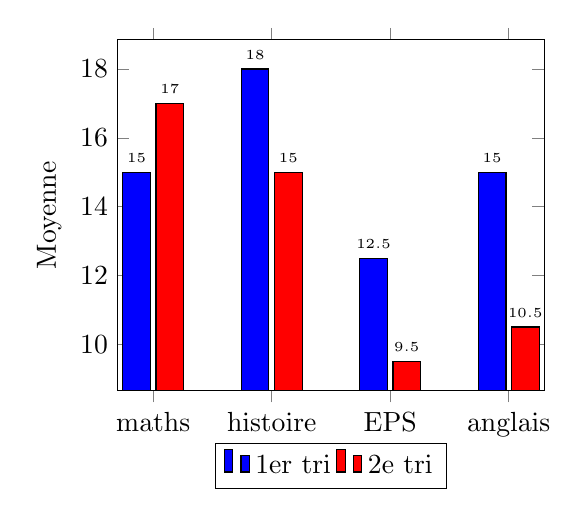
\begin{tikzpicture}
\begin{axis}[
	ytick={0,2,...,20},
	minor y tick num={0},
	ybar,
%	enlargelimits=0.15,
	legend style={at={(0.5,-0.15)},
			anchor=north, legend columns=-1},
	ylabel={Moyenne},
	symbolic x coords={{maths}, {histoire}, {EPS}, {anglais}},
	xtick=data,
	nodes near coords,
	every node near coord/.append style={font=\tiny},
	nodes near coords align={vertical},
	]
	
\addplot[ybar,fill=blue] coordinates {
	(maths,15)
	(histoire,18)
	(EPS,12.5)
	(anglais,15)
};

\addplot[ybar,fill=red] coordinates {
	(maths,17)
	(histoire,15)
	(EPS,9.5)
	(anglais,10.5)
};

\legend{1er tri, 2e tri}
\end{axis}
\end{tikzpicture}	
	
%\begin{tikzpicture}
%\begin{axis}[ 
%xbar, xmin=0,
%xlabel={Percentage \%},
%symbolic y coords={%
%	{Bloodstream Infection (BSI)},
%	{Surgical site infections (SSI)},
%	{Ventilator-associated pneumonia (VAP)},
%	{Urinary tract infection (UTI)},
%	Others},
%ytick=data,
%nodes near coords, 
%nodes near coords align={horizontal},
%ytick=data,
%]
%\addplot coordinates {
%	(14,{Bloodstream Infection (BSI)}) 
%	(17,{Surgical site infections (SSI)}) 
%	(14,{Ventilator-associated pneumonia (VAP)}) 
%	(33,{Urinary tract infection (UTI)})
%	(22,Others)};
%\end{axis}
%\end{tikzpicture}
\end{frame}

\begin{frame}
\frametitle{ACAR Omer (18/12/2000)}  
\framesubtitle{ }	

%
%	\begin{column}{0.35\textwidth}
%		\begin{block}{ACAR OMER}
%			\begin{itemize}
%				\item \date{18/12/2000}
%				\item Métier : Assureur
%				\item Orientation
%				\begin{enumerate}
%					\item 2$^nde$ GT
%					\item BPC
%				\end{enumerate}
%			\end{itemize}
%		\end{block}	
%		
%		
%	\end{column}
%	\begin{column}{0.15\textwidth}
%		\includegraphics[scale=0.5]{tof}
%	\end{column}
%	
%	\begin{column}{0.50\textwidth}
%		notes
%	\end{column}
%
\begin{columns}[onlytextwidth]

\vspace*{-.5cm}

\begin{column}{0.3\textwidth}
	\begin{center}
			\includegraphics[scale=0.8]{tof}
	\end{center}

	
	\begin{block}{Métier envisagé}
		Assureur
	\end{block}
	
	\begin{alertblock}{Orientation}
		\begin{enumerate}
			\item 2$^{de}$ GT
			\item BAC PRO COM
		\end{enumerate}
	\end{alertblock}
\end{column}	

\begin{column}{0.70\textwidth}
	
%	\begin{table}[]
%		\centering
%		\caption{My caption}
%		\label{my-label}
		\begin{center}
		
		\vspace*{-.7cm}	

		{\small \begin{tabular}{cccc}
			& Classe                       & \'Elève                      & Classement                   \\
			{\color[HTML]{00009B} Trimestre 1} & {\color[HTML]{00009B} 12,40} & {\color[HTML]{00009B} 10.52} & {\color[HTML]{00009B} 22/27} \\
			{\color[HTML]{FE0000} Trimestre 2} & {\color[HTML]{FE0000} 11,69} & {\color[HTML]{FE0000} 10.11} & {\color[HTML]{FE0000} 25/28} \\
			{\color[HTML]{34FF34} Trimestre 3} & {\color[HTML]{34FF34} 12,46} & {\color[HTML]{34FF34} 11.69} & {\color[HTML]{34FF34} 16/29}
		\end{tabular}}
		
	
%	\end{table}

\vspace*{-1cm}
	
\begin{tikzpicture}[label distance=.15cm,rotate=30,scale=.55]
\tkzKiviatDiagram[radial=7,lattice=4,gap=1,step=0.2,label space=1.2]%
{Maths,
	Histoire Géo,
	Français,
	EPS,
	SVT,
	Techno,
	Physique}
\tkzKiviatLine[thick,color=red](6.5,5,7.5,1,2.5,5, 15)
\tkzKiviatLine[thick,color=blue](15,16,13,18,11,7, 18)
\tkzKiviatGrad[prefix=,unity=5](0)   
\end{tikzpicture}

	\end{center}
	
\end{column}	

\end{columns}

\end{frame}


\end{document}


\begin{frame}
	\frametitle{}  
	\framesubtitle{}	
	
\end{frame}